\chapter{Analisis}
\label{chap:analisis}

Pada bab ini akan dijelaskan mengenai analisis pemanfaatan jsoup untuk mengambil data mahasiswa, dan analisis pemanfaatan JavaFX untuk membuat tampilan antarmuka pengguna.

\section{Analisis Pemanfaatan Jsoup}
Untuk mengambil data mahasiswa, diperlukan sumber data mahasiswa tersebut. Sumber data mahasiswa tersebut dapat diperoleh melalui Portal Akademik Mahasiswa. Portal Akademik Mahasiswa merupakan sebuah situs yang diperuntukkan bagi mahasiswa untuk mendapatkan informasi mengenai profil dan kegiatan akademik mahasiswa tersebut. Mahasiswa dapat mengakses Portal Akademik Mahasiswa melalui \textit{URL} \url{https://studentportal.unpar.ac.id/}. Untuk mengakses Portal Akademik Mahasiswa, mahasiswa harus melakukan \textit{login} menggunakan \textit{email} dan \textit{password} mahasiswa tersebut.

Pada halaman utama Portal Akademik Mahasiswa (Gambar \ref{fig:3_home}), terdapat beberapa menu yang dapat digunakan sebagai sumber data yaitu:

\begin{figure}[H]
	\centering
	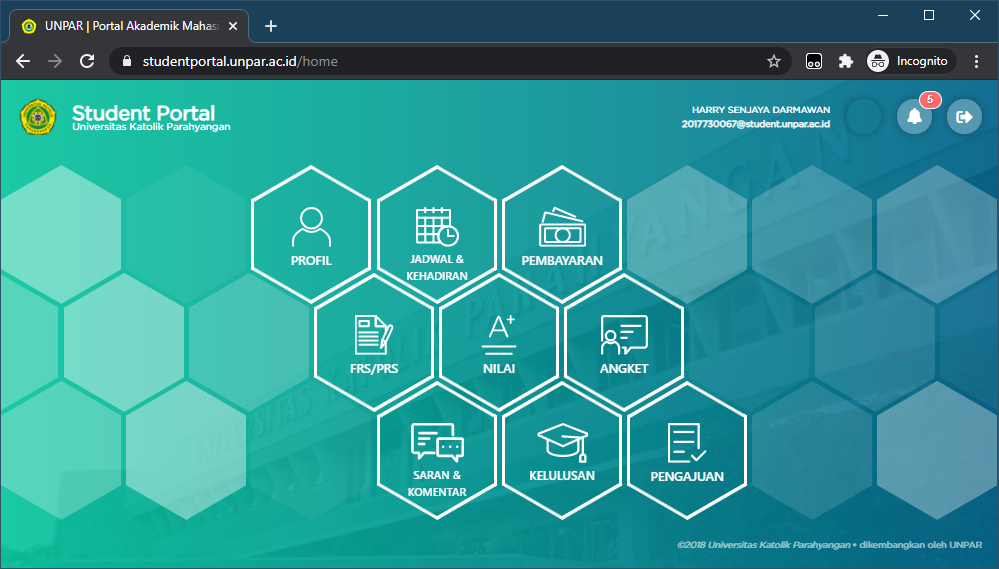
\includegraphics[scale=0.45]{Gambar/home.png}
	\caption{Halaman Utama Portal Akademik Mahasiswa} 
	\label{fig:3_home}
\end{figure}

\begin{enumerate}
    \item Profil\\
    \textbf{Profil}, merupakan halaman yang menampilkan data mengenai profil dari mahasiswa tersebut (Gambar \ref{fig:3_profil}).
    
    \begin{figure}[H]
    	\centering
    	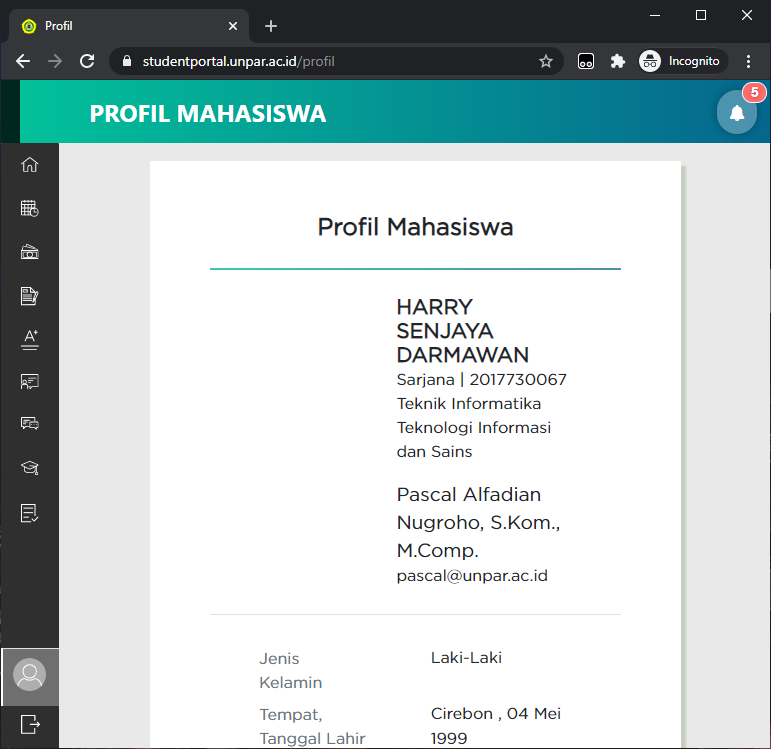
\includegraphics[scale=0.45]{Gambar/profil.png}
    	\caption{Halaman Profil} 
    	\label{fig:3_profil}
    \end{figure}
\end{enumerate}

